\clearpage
\subsection{Results from "dell" [df6407d], generated Sun Sep 25 23:06:58 CEST 2011}
\begin{verbatim}

Test aspects:

    compilation:
        compilation time measured by 'time' call
        only 'real' time is taken into account
        result is in seconds

    size:
        size of the binary measured by 'ls -k' call
        result is in kilobytes

    strip-size:
        size of the binary measured by 'ls -k' call after 'strip' call
        result is in kilobytes

    execution:
        execution time measured by 'time' call
        only 'real' time is taken into account
        result is in seconds

    valgrind:
        test is executed with valgrind call
        result is as A/D (S), where
        A - allocations
        D - deallocations
        S - global allocated size in bytes

    test name:
        test_NAME[_NUMBER], where NAME is test case name and NUMBER is count of event calls during the test
\end{verbatim}
\begin{center}
\line(1,0){750}
\end{center}
\begin{verbatim}

Environment statistics:

    generated: Sun Sep 25 23:06:58 CEST 2011
    code revision: df6407d
    hostname: "dell"
    operating system:  GNU/Linux
    processor: Intel(R) Core(TM)2 Duo CPU P8600 @ 2.40GHz
    free memory: 896Mb
    load average: 0.95 1.04 0.88 1/240 30884
\end{verbatim}
\begin{center}
\line(1,0){750}
\end{center}
\begin{verbatim}

All tests summary:

    real: 1329.65s (22:09.65)
    user: 1283.62s
    sys: 18.77s
    cpu: 97%
    average memory usage: 0K
    maximum resident set size: 0K
    number of times the process was swapped out of main memory: 0
    number of file system input: 1472
    number of file system outputs: 1046512
\end{verbatim}
\begin{center}
\line(1,0){750}
\end{center}
\begin{verbatim}
Results are presented by using table and two types of charts:

    table: contains results for each tested aspect and framework
    first type of chart: presents relative (0-100%) differents between individual framework and aspect
    second type of chart: presents each aspect individually using exact values returned during the test
\end{verbatim}
\begin{center}
\line(1,0){750}
\end{center}

\begin{landscape}
\begin{table}
\caption{"dell" [df6407d], g++-4.3.5 -m32/test transitions 1000000}
\centering
\begin{longtable}{| c | c |c |c |c |c |c |c |}
\hline
& CFsmBase& StateChart& MSM.favor\_runtime\_speed& MSM.favor\_compile\_time& QFsm.FavorExecutionSpeed& QFsm.FavorCompilationTime& QFsm.FavorDebugSize\\
\hline
compilation & 0.66s & 0.88s & 2.30s & 2.22s & 0.67s & 0.59s & 0.66s\\
\hline
size & 38K & 113K & 103K & 122K & 27K & 20K & 40K\\
\hline
strip-size & 22K & 46K & 34K & 38K & 10K & 10K & 18K\\
\hline
execution & 0.06s & 1.17s & 0.38s & 0.50s & 0.07s & 0.14s & 0.23s\\
\hline
valgrind & 0.06s & 1.17s & 0.38s & 0.50s & 0.07s & 0.14s & 0.23s\\
\hline
\multicolumn{8}{|c|}{\includegraphics[scale=0.8]{images/"results/dell"/"g++-4.3.5 -m32"/test_transitions_1000000_all.png}}\\
\hline
\end{longtable}
\end{table}
\end{landscape}
\newpage
\begin{table}
\centering
\begin{longtable}{| c | c |}
\hline
\includegraphics[scale=0.8]{images/"results/dell"/"g++-4.3.5 -m32"/test_transitions_1000000_compilation.png}& \includegraphics[scale=0.8]{images/"results/dell"/"g++-4.3.5 -m32"/test_transitions_1000000_size.png}\\
\hline
\includegraphics[scale=0.8]{images/"results/dell"/"g++-4.3.5 -m32"/test_transitions_1000000_strip-size.png}& \includegraphics[scale=0.8]{images/"results/dell"/"g++-4.3.5 -m32"/test_transitions_1000000_execution.png}\\
\hline
\includegraphics[scale=0.8]{images/"results/dell"/"g++-4.3.5 -m32"/test_transitions_1000000_valgrind.png}& \\ \hline
\end{longtable}
\end{table}
\begin{landscape}
\begin{table}
\caption{"dell" [df6407d], g++-4.3.5 -m32/test complex 1000000}
\centering
\begin{longtable}{| c | c |c |c |c |c |c |c |}
\hline
& CFsmBase& StateChart& MSM.favor\_runtime\_speed& MSM.favor\_compile\_time& QFsm.FavorExecutionSpeed& QFsm.FavorCompilationTime& QFsm.FavorDebugSize\\
\hline
compilation & 0.74s & 1.58s & 13.19s & 9.40s & 26.27s & 1.95s & 1.83s\\
\hline
size & 52K & 353K & 961K & 1177K & 453K & 410K & 177K\\
\hline
strip-size & 30K & 122K & 114K & 158K & 30K & 50K & 66K\\
\hline
execution & 0.19s & 1.65s & 0.57s & 0.67s & 0.08s & 0.45s & 1.05s\\
\hline
valgrind & 0.19s & 1.65s & 0.57s & 0.67s & 0.08s & 0.45s & 1.05s\\
\hline
\multicolumn{8}{|c|}{\includegraphics[scale=0.8]{images/"results/dell"/"g++-4.3.5 -m32"/test_complex_1000000_all.png}}\\
\hline
\end{longtable}
\end{table}
\end{landscape}
\newpage
\begin{table}
\centering
\begin{longtable}{| c | c |}
\hline
\includegraphics[scale=0.8]{images/"results/dell"/"g++-4.3.5 -m32"/test_complex_1000000_compilation.png}& \includegraphics[scale=0.8]{images/"results/dell"/"g++-4.3.5 -m32"/test_complex_1000000_size.png}\\
\hline
\includegraphics[scale=0.8]{images/"results/dell"/"g++-4.3.5 -m32"/test_complex_1000000_strip-size.png}& \includegraphics[scale=0.8]{images/"results/dell"/"g++-4.3.5 -m32"/test_complex_1000000_execution.png}\\
\hline
\includegraphics[scale=0.8]{images/"results/dell"/"g++-4.3.5 -m32"/test_complex_1000000_valgrind.png}& \\ \hline
\end{longtable}
\end{table}
\begin{landscape}
\begin{table}
\caption{"dell" [df6407d], g++-4.3.5 -m32 -O1 -DNDEBUG/test transitions 1000000}
\centering
\begin{longtable}{| c | c |c |c |c |c |c |c |}
\hline
& CFsmBase& StateChart& MSM.favor\_runtime\_speed& MSM.favor\_compile\_time& QFsm.FavorExecutionSpeed& QFsm.FavorCompilationTime& QFsm.FavorDebugSize\\
\hline
compilation & 1.21s & 1.06s & 2.28s & 2.33s & 0.54s & 0.48s & 0.63s\\
\hline
size & 27K & 32K & 35K & 36K & 11K & 9K & 21K\\
\hline
strip-size & 18K & 18K & 18K & 18K & 6K & 6K & 14K\\
\hline
execution & 0.08s & 0.14s & 0.02s & 0.03s & 0.01s & 0.01s & 0.01s\\
\hline
valgrind & 0.08s & 0.14s & 0.02s & 0.03s & 0.01s & 0.01s & 0.01s\\
\hline
\multicolumn{8}{|c|}{\includegraphics[scale=0.8]{images/"results/dell"/"g++-4.3.5 -m32 -O1 -DNDEBUG"/test_transitions_1000000_all.png}}\\
\hline
\end{longtable}
\end{table}
\end{landscape}
\newpage
\begin{table}
\centering
\begin{longtable}{| c | c |}
\hline
\includegraphics[scale=0.8]{images/"results/dell"/"g++-4.3.5 -m32 -O1 -DNDEBUG"/test_transitions_1000000_compilation.png}& \includegraphics[scale=0.8]{images/"results/dell"/"g++-4.3.5 -m32 -O1 -DNDEBUG"/test_transitions_1000000_size.png}\\
\hline
\includegraphics[scale=0.8]{images/"results/dell"/"g++-4.3.5 -m32 -O1 -DNDEBUG"/test_transitions_1000000_strip-size.png}& \includegraphics[scale=0.8]{images/"results/dell"/"g++-4.3.5 -m32 -O1 -DNDEBUG"/test_transitions_1000000_execution.png}\\
\hline
\includegraphics[scale=0.8]{images/"results/dell"/"g++-4.3.5 -m32 -O1 -DNDEBUG"/test_transitions_1000000_valgrind.png}& \\ \hline
\end{longtable}
\end{table}
\begin{landscape}
\begin{table}
\caption{"dell" [df6407d], g++-4.3.5 -m32 -O1 -DNDEBUG/test complex 1000000}
\centering
\begin{longtable}{| c | c |c |c |c |c |c |c |}
\hline
& CFsmBase& StateChart& MSM.favor\_runtime\_speed& MSM.favor\_compile\_time& QFsm.FavorExecutionSpeed& QFsm.FavorCompilationTime& QFsm.FavorDebugSize\\
\hline
compilation & 0.97s & 1.73s & 13.14s & 9.51s & 26.02s & 1.68s & 2.20s\\
\hline
size & 35K & 67K & 248K & 289K & 88K & 22K & 74K\\
\hline
strip-size & 22K & 34K & 38K & 54K & 10K & 10K & 42K\\
\hline
execution & 0.15s & 0.13s & 0.05s & 0.06s & 0.01s & 0.01s & 0.06s\\
\hline
valgrind & 0.15s & 0.13s & 0.05s & 0.06s & 0.01s & 0.01s & 0.06s\\
\hline
\multicolumn{8}{|c|}{\includegraphics[scale=0.8]{images/"results/dell"/"g++-4.3.5 -m32 -O1 -DNDEBUG"/test_complex_1000000_all.png}}\\
\hline
\end{longtable}
\end{table}
\end{landscape}
\newpage
\begin{table}
\centering
\begin{longtable}{| c | c |}
\hline
\includegraphics[scale=0.8]{images/"results/dell"/"g++-4.3.5 -m32 -O1 -DNDEBUG"/test_complex_1000000_compilation.png}& \includegraphics[scale=0.8]{images/"results/dell"/"g++-4.3.5 -m32 -O1 -DNDEBUG"/test_complex_1000000_size.png}\\
\hline
\includegraphics[scale=0.8]{images/"results/dell"/"g++-4.3.5 -m32 -O1 -DNDEBUG"/test_complex_1000000_strip-size.png}& \includegraphics[scale=0.8]{images/"results/dell"/"g++-4.3.5 -m32 -O1 -DNDEBUG"/test_complex_1000000_execution.png}\\
\hline
\includegraphics[scale=0.8]{images/"results/dell"/"g++-4.3.5 -m32 -O1 -DNDEBUG"/test_complex_1000000_valgrind.png}& \\ \hline
\end{longtable}
\end{table}
\begin{landscape}
\begin{table}
\caption{"dell" [df6407d], g++-4.3.5 -m32 -O2 -DNDEBUG/test transitions 1000000}
\centering
\begin{longtable}{| c | c |c |c |c |c |c |c |}
\hline
& CFsmBase& StateChart& MSM.favor\_runtime\_speed& MSM.favor\_compile\_time& QFsm.FavorExecutionSpeed& QFsm.FavorCompilationTime& QFsm.FavorDebugSize\\
\hline
compilation & 0.93s & 1.20s & 2.42s & 2.41s & 0.54s & 0.50s & 0.74s\\
\hline
size & 27K & 31K & 31K & 33K & 11K & 9K & 21K\\
\hline
strip-size & 18K & 18K & 18K & 18K & 6K & 6K & 14K\\
\hline
execution & 0.05s & 0.12s & 0.01s & 0.02s & 0.00s & 0.00s & 0.01s\\
\hline
valgrind & 0.05s & 0.12s & 0.01s & 0.02s & 0.00s & 0.00s & 0.01s\\
\hline
\multicolumn{8}{|c|}{\includegraphics[scale=0.8]{images/"results/dell"/"g++-4.3.5 -m32 -O2 -DNDEBUG"/test_transitions_1000000_all.png}}\\
\hline
\end{longtable}
\end{table}
\end{landscape}
\newpage
\begin{table}
\centering
\begin{longtable}{| c | c |}
\hline
\includegraphics[scale=0.8]{images/"results/dell"/"g++-4.3.5 -m32 -O2 -DNDEBUG"/test_transitions_1000000_compilation.png}& \includegraphics[scale=0.8]{images/"results/dell"/"g++-4.3.5 -m32 -O2 -DNDEBUG"/test_transitions_1000000_size.png}\\
\hline
\includegraphics[scale=0.8]{images/"results/dell"/"g++-4.3.5 -m32 -O2 -DNDEBUG"/test_transitions_1000000_strip-size.png}& \includegraphics[scale=0.8]{images/"results/dell"/"g++-4.3.5 -m32 -O2 -DNDEBUG"/test_transitions_1000000_execution.png}\\
\hline
\includegraphics[scale=0.8]{images/"results/dell"/"g++-4.3.5 -m32 -O2 -DNDEBUG"/test_transitions_1000000_valgrind.png}& \\ \hline
\end{longtable}
\end{table}
\begin{landscape}
\begin{table}
\caption{"dell" [df6407d], g++-4.3.5 -m32 -O2 -DNDEBUG/test complex 1000000}
\centering
\begin{longtable}{| c | c |c |c |c |c |c |c |}
\hline
& CFsmBase& StateChart& MSM.favor\_runtime\_speed& MSM.favor\_compile\_time& QFsm.FavorExecutionSpeed& QFsm.FavorCompilationTime& QFsm.FavorDebugSize\\
\hline
compilation & 1.08s & 2.09s & 12.99s & 9.84s & 25.50s & 1.78s & 2.61s\\
\hline
size & 35K & 65K & 226K & 265K & 92K & 22K & 74K\\
\hline
strip-size & 22K & 34K & 34K & 50K & 14K & 10K & 42K\\
\hline
execution & 0.15s & 0.11s & 0.01s & 0.02s & 0.00s & 0.01s & 0.04s\\
\hline
valgrind & 0.15s & 0.11s & 0.01s & 0.02s & 0.00s & 0.01s & 0.04s\\
\hline
\multicolumn{8}{|c|}{\includegraphics[scale=0.8]{images/"results/dell"/"g++-4.3.5 -m32 -O2 -DNDEBUG"/test_complex_1000000_all.png}}\\
\hline
\end{longtable}
\end{table}
\end{landscape}
\newpage
\begin{table}
\centering
\begin{longtable}{| c | c |}
\hline
\includegraphics[scale=0.8]{images/"results/dell"/"g++-4.3.5 -m32 -O2 -DNDEBUG"/test_complex_1000000_compilation.png}& \includegraphics[scale=0.8]{images/"results/dell"/"g++-4.3.5 -m32 -O2 -DNDEBUG"/test_complex_1000000_size.png}\\
\hline
\includegraphics[scale=0.8]{images/"results/dell"/"g++-4.3.5 -m32 -O2 -DNDEBUG"/test_complex_1000000_strip-size.png}& \includegraphics[scale=0.8]{images/"results/dell"/"g++-4.3.5 -m32 -O2 -DNDEBUG"/test_complex_1000000_execution.png}\\
\hline
\includegraphics[scale=0.8]{images/"results/dell"/"g++-4.3.5 -m32 -O2 -DNDEBUG"/test_complex_1000000_valgrind.png}& \\ \hline
\end{longtable}
\end{table}
\begin{landscape}
\begin{table}
\caption{"dell" [df6407d], g++-4.3.5 -m32 -Os -DNDEBUG/test transitions 1000000}
\centering
\begin{longtable}{| c | c |c |c |c |c |c |c |}
\hline
& CFsmBase& StateChart& MSM.favor\_runtime\_speed& MSM.favor\_compile\_time& QFsm.FavorExecutionSpeed& QFsm.FavorCompilationTime& QFsm.FavorDebugSize\\
\hline
compilation & 0.92s & 1.01s & 2.29s & 2.31s & 0.57s & 0.49s & 0.63s\\
\hline
size & 23K & 28K & 28K & 29K & 11K & 9K & 17K\\
\hline
strip-size & 14K & 14K & 14K & 14K & 6K & 6K & 10K\\
\hline
execution & 0.05s & 0.16s & 0.02s & 0.02s & 0.00s & 0.00s & 0.01s\\
\hline
valgrind & 0.05s & 0.16s & 0.02s & 0.02s & 0.00s & 0.00s & 0.01s\\
\hline
\multicolumn{8}{|c|}{\includegraphics[scale=0.8]{images/"results/dell"/"g++-4.3.5 -m32 -Os -DNDEBUG"/test_transitions_1000000_all.png}}\\
\hline
\end{longtable}
\end{table}
\end{landscape}
\newpage
\begin{table}
\centering
\begin{longtable}{| c | c |}
\hline
\includegraphics[scale=0.8]{images/"results/dell"/"g++-4.3.5 -m32 -Os -DNDEBUG"/test_transitions_1000000_compilation.png}& \includegraphics[scale=0.8]{images/"results/dell"/"g++-4.3.5 -m32 -Os -DNDEBUG"/test_transitions_1000000_size.png}\\
\hline
\includegraphics[scale=0.8]{images/"results/dell"/"g++-4.3.5 -m32 -Os -DNDEBUG"/test_transitions_1000000_strip-size.png}& \includegraphics[scale=0.8]{images/"results/dell"/"g++-4.3.5 -m32 -Os -DNDEBUG"/test_transitions_1000000_execution.png}\\
\hline
\includegraphics[scale=0.8]{images/"results/dell"/"g++-4.3.5 -m32 -Os -DNDEBUG"/test_transitions_1000000_valgrind.png}& \\ \hline
\end{longtable}
\end{table}
\begin{landscape}
\begin{table}
\caption{"dell" [df6407d], g++-4.3.5 -m32 -Os -DNDEBUG/test complex 1000000}
\centering
\begin{longtable}{| c | c |c |c |c |c |c |c |}
\hline
& CFsmBase& StateChart& MSM.favor\_runtime\_speed& MSM.favor\_compile\_time& QFsm.FavorExecutionSpeed& QFsm.FavorCompilationTime& QFsm.FavorDebugSize\\
\hline
compilation & 1.05s & 1.68s & 12.93s & 9.45s & 26.04s & 1.71s & 2.25s\\
\hline
size & 30K & 59K & 214K & 252K & 88K & 22K & 63K\\
\hline
strip-size & 18K & 26K & 22K & 34K & 10K & 10K & 34K\\
\hline
execution & 0.17s & 0.17s & 0.02s & 0.03s & 0.01s & 0.01s & 0.08s\\
\hline
valgrind & 0.17s & 0.17s & 0.02s & 0.03s & 0.01s & 0.01s & 0.08s\\
\hline
\multicolumn{8}{|c|}{\includegraphics[scale=0.8]{images/"results/dell"/"g++-4.3.5 -m32 -Os -DNDEBUG"/test_complex_1000000_all.png}}\\
\hline
\end{longtable}
\end{table}
\end{landscape}
\newpage
\begin{table}
\centering
\begin{longtable}{| c | c |}
\hline
\includegraphics[scale=0.8]{images/"results/dell"/"g++-4.3.5 -m32 -Os -DNDEBUG"/test_complex_1000000_compilation.png}& \includegraphics[scale=0.8]{images/"results/dell"/"g++-4.3.5 -m32 -Os -DNDEBUG"/test_complex_1000000_size.png}\\
\hline
\includegraphics[scale=0.8]{images/"results/dell"/"g++-4.3.5 -m32 -Os -DNDEBUG"/test_complex_1000000_strip-size.png}& \includegraphics[scale=0.8]{images/"results/dell"/"g++-4.3.5 -m32 -Os -DNDEBUG"/test_complex_1000000_execution.png}\\
\hline
\includegraphics[scale=0.8]{images/"results/dell"/"g++-4.3.5 -m32 -Os -DNDEBUG"/test_complex_1000000_valgrind.png}& \\ \hline
\end{longtable}
\end{table}
\begin{landscape}
\begin{table}
\caption{"dell" [df6407d], g++-4.3.5 -m32 -g -O0/test transitions 1000000}
\centering
\begin{longtable}{| c | c |c |c |c |c |c |c |}
\hline
& CFsmBase& StateChart& MSM.favor\_runtime\_speed& MSM.favor\_compile\_time& QFsm.FavorExecutionSpeed& QFsm.FavorCompilationTime& QFsm.FavorDebugSize\\
\hline
compilation & 0.75s & 1.02s & 2.44s & 2.48s & 0.72s & 0.70s & 0.74s\\
\hline
size & 165K & 437K & 664K & 754K & 189K & 119K & 187K\\
\hline
strip-size & 22K & 46K & 34K & 38K & 10K & 10K & 18K\\
\hline
execution & 0.06s & 1.19s & 0.39s & 0.49s & 0.07s & 0.17s & 0.24s\\
\hline
valgrind & 0.06s & 1.19s & 0.39s & 0.49s & 0.07s & 0.17s & 0.24s\\
\hline
\multicolumn{8}{|c|}{\includegraphics[scale=0.8]{images/"results/dell"/"g++-4.3.5 -m32 -g -O0"/test_transitions_1000000_all.png}}\\
\hline
\end{longtable}
\end{table}
\end{landscape}
\newpage
\begin{table}
\centering
\begin{longtable}{| c | c |}
\hline
\includegraphics[scale=0.8]{images/"results/dell"/"g++-4.3.5 -m32 -g -O0"/test_transitions_1000000_compilation.png}& \includegraphics[scale=0.8]{images/"results/dell"/"g++-4.3.5 -m32 -g -O0"/test_transitions_1000000_size.png}\\
\hline
\includegraphics[scale=0.8]{images/"results/dell"/"g++-4.3.5 -m32 -g -O0"/test_transitions_1000000_strip-size.png}& \includegraphics[scale=0.8]{images/"results/dell"/"g++-4.3.5 -m32 -g -O0"/test_transitions_1000000_execution.png}\\
\hline
\includegraphics[scale=0.8]{images/"results/dell"/"g++-4.3.5 -m32 -g -O0"/test_transitions_1000000_valgrind.png}& \\ \hline
\end{longtable}
\end{table}
\begin{landscape}
\begin{table}
\caption{"dell" [df6407d], g++-4.3.5 -m32 -g -O0/test complex 1000000}
\centering
\begin{longtable}{| c | c |c |c |c |c |c |c |}
\hline
& CFsmBase& StateChart& MSM.favor\_runtime\_speed& MSM.favor\_compile\_time& QFsm.FavorExecutionSpeed& QFsm.FavorCompilationTime& QFsm.FavorDebugSize\\
\hline
compilation & 0.84s & 1.92s & 17.95s & 14.25s & 34.19s & 2.71s & 2.18s\\
\hline
size & 206K & 1298K & 23458K & 29225K & 13678K & 7709K & 838K\\
\hline
strip-size & 30K & 122K & 114K & 158K & 30K & 50K & 66K\\
\hline
execution & 0.21s & 1.64s & 0.56s & 0.67s & 0.09s & 0.46s & 1.11s\\
\hline
valgrind & 0.21s & 1.64s & 0.56s & 0.67s & 0.09s & 0.46s & 1.11s\\
\hline
\multicolumn{8}{|c|}{\includegraphics[scale=0.8]{images/"results/dell"/"g++-4.3.5 -m32 -g -O0"/test_complex_1000000_all.png}}\\
\hline
\end{longtable}
\end{table}
\end{landscape}
\newpage
\begin{table}
\centering
\begin{longtable}{| c | c |}
\hline
\includegraphics[scale=0.8]{images/"results/dell"/"g++-4.3.5 -m32 -g -O0"/test_complex_1000000_compilation.png}& \includegraphics[scale=0.8]{images/"results/dell"/"g++-4.3.5 -m32 -g -O0"/test_complex_1000000_size.png}\\
\hline
\includegraphics[scale=0.8]{images/"results/dell"/"g++-4.3.5 -m32 -g -O0"/test_complex_1000000_strip-size.png}& \includegraphics[scale=0.8]{images/"results/dell"/"g++-4.3.5 -m32 -g -O0"/test_complex_1000000_execution.png}\\
\hline
\includegraphics[scale=0.8]{images/"results/dell"/"g++-4.3.5 -m32 -g -O0"/test_complex_1000000_valgrind.png}& \\ \hline
\end{longtable}
\end{table}
\begin{landscape}
\begin{table}
\caption{"dell" [df6407d], g++-4.3.5 -m32 -g -O2/test transitions 1000000}
\centering
\begin{longtable}{| c | c |c |c |c |c |c |c |}
\hline
& CFsmBase& StateChart& MSM.favor\_runtime\_speed& MSM.favor\_compile\_time& QFsm.FavorExecutionSpeed& QFsm.FavorCompilationTime& QFsm.FavorDebugSize\\
\hline
compilation & 1.05s & 1.49s & 2.65s & 2.67s & 0.75s & 0.69s & 0.93s\\
\hline
size & 158K & 313K & 417K & 453K & 142K & 92K & 154K\\
\hline
strip-size & 18K & 34K & 22K & 22K & 10K & 6K & 14K\\
\hline
execution & 0.05s & 0.25s & 0.01s & 0.02s & 0.00s & 0.00s & 0.01s\\
\hline
valgrind & 0.05s & 0.25s & 0.01s & 0.02s & 0.00s & 0.00s & 0.01s\\
\hline
\multicolumn{8}{|c|}{\includegraphics[scale=0.8]{images/"results/dell"/"g++-4.3.5 -m32 -g -O2"/test_transitions_1000000_all.png}}\\
\hline
\end{longtable}
\end{table}
\end{landscape}
\newpage
\begin{table}
\centering
\begin{longtable}{| c | c |}
\hline
\includegraphics[scale=0.8]{images/"results/dell"/"g++-4.3.5 -m32 -g -O2"/test_transitions_1000000_compilation.png}& \includegraphics[scale=0.8]{images/"results/dell"/"g++-4.3.5 -m32 -g -O2"/test_transitions_1000000_size.png}\\
\hline
\includegraphics[scale=0.8]{images/"results/dell"/"g++-4.3.5 -m32 -g -O2"/test_transitions_1000000_strip-size.png}& \includegraphics[scale=0.8]{images/"results/dell"/"g++-4.3.5 -m32 -g -O2"/test_transitions_1000000_execution.png}\\
\hline
\includegraphics[scale=0.8]{images/"results/dell"/"g++-4.3.5 -m32 -g -O2"/test_transitions_1000000_valgrind.png}& \\ \hline
\end{longtable}
\end{table}
\begin{landscape}
\begin{table}
\caption{"dell" [df6407d], g++-4.3.5 -m32 -g -O2/test complex 1000000}
\centering
\begin{longtable}{| c | c |c |c |c |c |c |c |}
\hline
& CFsmBase& StateChart& MSM.favor\_runtime\_speed& MSM.favor\_compile\_time& QFsm.FavorExecutionSpeed& QFsm.FavorCompilationTime& QFsm.FavorDebugSize\\
\hline
compilation & 1.30s & 2.76s & 18.15s & 14.20s & 34.16s & 2.55s & 3.36s\\
\hline
size & 199K & 764K & 11452K & 14355K & 9349K & 3709K & 738K\\
\hline
strip-size & 26K & 70K & 58K & 78K & 14K & 14K & 46K\\
\hline
execution & 0.15s & 0.34s & 0.01s & 0.02s & 0.00s & 0.01s & 0.06s\\
\hline
valgrind & 0.15s & 0.34s & 0.01s & 0.02s & 0.00s & 0.01s & 0.06s\\
\hline
\multicolumn{8}{|c|}{\includegraphics[scale=0.8]{images/"results/dell"/"g++-4.3.5 -m32 -g -O2"/test_complex_1000000_all.png}}\\
\hline
\end{longtable}
\end{table}
\end{landscape}
\newpage
\begin{table}
\centering
\begin{longtable}{| c | c |}
\hline
\includegraphics[scale=0.8]{images/"results/dell"/"g++-4.3.5 -m32 -g -O2"/test_complex_1000000_compilation.png}& \includegraphics[scale=0.8]{images/"results/dell"/"g++-4.3.5 -m32 -g -O2"/test_complex_1000000_size.png}\\
\hline
\includegraphics[scale=0.8]{images/"results/dell"/"g++-4.3.5 -m32 -g -O2"/test_complex_1000000_strip-size.png}& \includegraphics[scale=0.8]{images/"results/dell"/"g++-4.3.5 -m32 -g -O2"/test_complex_1000000_execution.png}\\
\hline
\includegraphics[scale=0.8]{images/"results/dell"/"g++-4.3.5 -m32 -g -O2"/test_complex_1000000_valgrind.png}& \\ \hline
\end{longtable}
\end{table}
